 \documentclass[10pt,a4paper]{article}

% === PAQUETES === (((
\usepackage{amsmath}
\usepackage[shortlabels]{enumitem}
\usepackage{amsfonts}
\usepackage{ragged2e}
\usepackage{subfigure}
\usepackage{amssymb}
\usepackage{slashbox}
\usepackage{multirow}
\usepackage{multicol}
\usepackage{fontspec}
\usepackage{fullpage}
\usepackage{graphicx}
\usepackage{titlesec} 
% \usepackage{setspace}
\usepackage{dsfont}
% \usepackage{bookmark}
% )))

% === TIPOGRAFÍA === (((
\setmainfont[
  BoldFont       = bodonibi,
	ItalicFont     = Century modern italic2.ttf,
	BoldItalicFont = bodonibi,
	SmallCapsFont  = lmromancaps10-regular.otf
]{Century_modern.ttf}
% )))

% === COMANDOS === (((
\newcommand{\dis}{\displaystyle}
\newcommand{\qed}{\hspace{0.5cm}\rule{0.16cm}{0.4cm}}
\newcommand{\micita}[1]{\([\)\cite{#1}\(]\)}
\newcommand{\operator}[1]{\mathop{\vphantom{\sum}\mathchoice{ \vcenter{\hbox{\huge $#1$}} }
{\vcenter{ \hbox{\Large $#1$}} }{#1}{#1}}\displaylimits}
\newcommand{\suma}{\operator{ 
\includegraphics[scale=0.09]{IMAGENES/Sigma.png}} }
\DeclareSymbolFont{italics}{\encodingdefault}{\rmdefault}{m}{it}
\DeclareSymbolFontAlphabet{\mathit}{italics}
\ExplSyntaxOn
\int_step_inline:nnnn { `A } { 1 } { `Z }
 {  \exp_args:Nf \DeclareMathSymbol{\char_generate:nn{#1}{11}}{\mathalpha}{italics}{#1} }
\int_step_inline:nnnn { `a } { 1 } { `z } {  \exp_args:Nf \DeclareMathSymbol{\char_generate:nn{#1}{11}}{\mathalpha}{italics}{#1}}
\ExplSyntaxOff
% )))

% === SECCIONES === (((
\titleformat*{\section}{\large\normalfont\bfseries}
\titleformat*{\subsection}{\large\itshape \centering}
% \setcounter{secnumdepth}{0}
\renewcommand*{\contentsname}{\large\textbf{CONTENIDOS.}}
\usepackage[nottoc,numbib]{tocbibind}
\renewcommand{\refname}{REFERENCIAS.}
\renewcommand{\tablename}{Tabla}
\renewcommand{\figurename}{Figura}
% )))

% === PORTADA === (((
% \pagestyle{empty}
\newcommand{\portada}{
\addfontfeature{LetterSpace=-5}
  \begin{titlepage}
  \centering
  \begin{figure}
    \centering
    
\includegraphics[scale=0.5]{IMAGENES/logo_uaa.png}  
  \end{figure}
  {\bfseries\Large\MakeUppercase{\textit{Universidad Autónoma de Aguascalientes.}} \par}
  \vspace{1cm}
  {\Large Centro de Ciencias Básicas. \vspace{0.5cm}\\[2mm]
  Departamento de Matemáticas y Física.\vspace{0.5cm}\\[2mm]
  Licenciatura en Matemáticas Aplicadas.\vspace{0.5cm}\\[2mm]
  Práctica 6.\par}
  \vspace{1.5cm}
  {\bfseries\Huge Experimento de Young. \par} % title
  \vspace{1.5cm}
  {\itshape\Large Óptica. \\Prof. Mariana Alfaro Gómez.\par}
  % {\itshape\Large Variable Compleja I. \\Prof. Fausto Arturo Contreras Rosales.\par}
  % {\itshape\Large Métodos Numéricos II. \\Prof. Manuel Ramírez Aranda.\par}
  % {\itshape\Large Diseño de Experimentos. \\Prof. Angélica Hernández Quintero.\par}
  % {\itshape\Large Filosofía de la Investigación Científica. \\Prof. Jesús Mariano Rodríguez Muñoz.\par}
  \vfill
  % {\Large \textit{Por Erick I. Rodríguez Juárez.}\par}
		\begin{flushleft}
		\Large
		Alumnos:\\
		\textit{Carlos Francisco Guzmán Barba.}\\
		\textit{Erick Ignacio Rodríguez Juárez.}\\
		\textit{Manuel Alejandro Siller Landin.}
		\end{flushleft}
	% {}  % {\Large \textit{Por Erick I. Rodríguez Juárez.}\par}
  \vfill
		\begin{flushright}
		{\Large Realización: 2\(/\)05\(/\)22. \par} % date
		{\Large Entrega: 16\(/\)05\(/\)22. \par} % date
		\end{flushright}
  \end{titlepage} 
	% \thispagestyle{empty}
	% \doublespacing
	% \tableofcontents
	% \singlespacing
	% \newpage
} 
% )))

\begin{document}

\portada

\section{RESUMEN.} % (((
% )))

\section{INTRODUCCIÓN.} % (((

% )))

\section{METODOLOGÍA.} % (((
% )))

\section{RESULTADOS.} % (((
% )))

  La incertidumbre del Vernier es de $ \dfrac{0.01 cm}{2}=0.005 cm $
	 
	 La incertidumbre del banco óptico es de $ \dfrac{0.1 cm}{2}=0.05 cm $
	 
	 
	 Durante el experimento, se tenían los siguientes datos ``fijos$"$:
	 
	 \begin{itemize}
	 	\item La distancia $ D $ entre la doble rendija y la pantalla era $ D=(90\pm 0.05) cm$
	 	\item La longitud de la onda del láser empleado era de $ \lambda=650 nm=6.5\times 10^{-5}cm $
	 \end{itemize}
 
 	Luego, para dos máximos de interferencia elegidos $ (m_1, m_2) $ en la pantalla, y considerando un ancho de rendija $ a $ separadas una distancia $ d $, la distancia $ y $ entre tales máximos elegidos se muestran en la siguiente tabla \ref{tab:distancias}
 	
 	\begin{table}[!htb]
 		\centering
 		\caption{Distancias entre máximos observados}
 		\begin{tabular}{|c|c|c|}
 			\hline
 			\backslashbox{$ a, d $ (mm)}{$ (m_1,m_2) $}& $ (0,2) $ & $ (0,4) $ \\
 			\hline
 			$ a=0.04 $ & \multirow{2}{*}{$ (0.395\pm 0.005) cm $} & \multirow{2}{*}{$ (0.845\pm 0.005) cm $} \\ 		
 			$ d=0.25 $ &  & \\ 
 			\hline
 			$ a=0.08 $& \multirow{2}{*}{$ (0.380\pm 0.005) cm $} & \multirow{2}{*}{$ (0.870\pm 0.005) cm $} \\
 			$ d=0.25 $&  &  \\
 			\hline
 			$ a=0.04 $          & \multirow{2}{*}{$ (0.215\pm 0.005) cm $} & \multirow{2}{*}{$ (0.430\pm 0.005) cm $} \\ 		
 			$ d=0.5\phantom{0} $&  &  \\	
 			\hline
 			$ a=0.08 $           & \multirow{2}{*}{$ (0.180 \pm 0.005) cm $} & \multirow{2}{*}{$ (0.420 \pm 0.005) cm $} \\
 			$ d=0.5\phantom{0} $ &  &  \\
 			\hline
 		\end{tabular}
 		\label{tab:distancias}
 	\end{table}
 	
  	Haciendo uso de la ecuación \ref{}, para los mismos valores anteriores se tienen las siguientes distancias teóricas (tabla \ref{tab:disteo} )
 	
 	\begin{table}[!htb]
 		\centering
 		\caption{Distancias teóricas para los máximos}
 		\begin{tabular}{|c|c|c|}
 			\hline
 			$ d $ (mm) & \multicolumn{2}{c|}{$ y_m $ (cm)}  \\
 			\hline
 			0.25 & $ y_2=0.4680\pm 0.0002 $ & $ y_4=0.9360\pm0.0005 $ \\
 			\hline
 			0.5 & $ y_2=0.2340\pm 0.0001 $ & $ y_4=0.4680\pm0.0002 $  \\
 			\hline
 		\end{tabular}
 		\label{tab:disteo}
 	\end{table}
 	
 	A continuación, en la tabla \ref{tab:errores} se calculan los errores absolutos y relativos de las mediciones obtenidas
 	
 	\begin{table}[!htb]
 		\centering
 		\caption{Errores absolutos y relativos}
 		\begin{tabular}{|c|c|c|c|c|}
 			\hline
 			$ a, d $ (mm) & $ y_m $ observado (cm) & $ y_m $ teórico (cm) & Error absoluto (cm) & Error relativo (\%)  \\
 			\hline
 			$ a=0.04 $          & $y_2=0.395\pm 0.005 $ & $y_2=0.4680\pm0.0002 $ & $ 0.073 $ & $ 15.59 $ \\ \cline{2-5}
 			$ d=0.25 $          & $y_4=0.845\pm 0.005 $ & $y_4=0.9360\pm0.0005 $ & $ 0.091 $ & $ \phantom{0}9.72 $ \\ \hline
 			$ a=0.08 $          & $y_2=0.380\pm 0.005 $ & $y_2=0.4680\pm0.0002 $ & $ 0.088 $ & $ 18.80 $ \\ \cline{2-5}
 			$ d=0.25 $          & $y_4=0.870\pm 0.005 $ & $y_4=0.9360\pm0.0005 $ & $ 0.066 $ & $ \phantom{0}7.05 $ \\ \hline
 			$ a=0.04 $          & $y_2=0.215\pm 0.005 $ & $y_2=0.2340\pm0.0001 $ & $ 0.019 $ & $ \phantom{0}8.11 $ \\ \cline{2-5}
 			$ d=0.5\phantom{0} $& $y_4=0.430\pm 0.005 $ & $y_4=0.4680\pm0.0002 $ & $ 0.038 $ & $ \phantom{0}8.11 $ \\ \hline
 			$ a=0.08 $          & $y_2=0.180\pm 0.005 $ & $y_2=0.2340\pm0.0001 $ & $ 0.054 $ & $ 23.07 $ \\ \cline{2-5}
 			$ d=0.5\phantom{0} $& $y_4=0.420\pm 0.005 $ & $y_4=0.4680\pm0.0002 $ & $ 0.048 $ & $ 10.25 $ \\ \hline
 		\end{tabular} 
 		\label{tab:errores}
 	\end{table}
 	 
	\begin{figure}[htbp!]
		\centering
		\subfloat[Foto de la rendija]{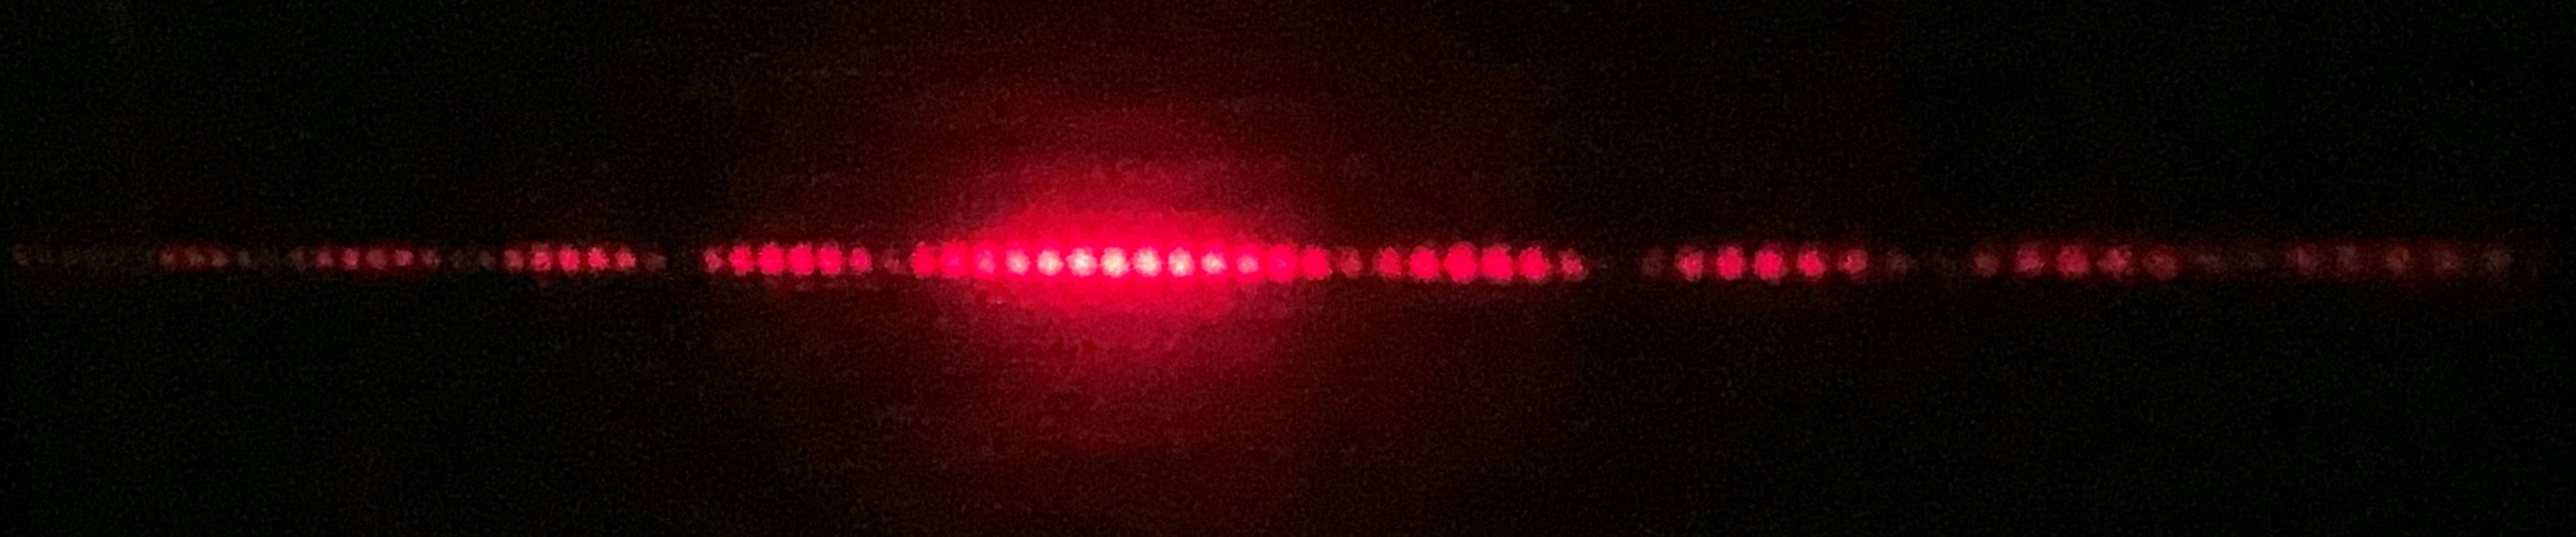
\includegraphics[width=1\textwidth]{04_y_25.jpg}\label{fig:A1}}
		\hfill
		\subfloat[Patrón de irradiancia experimental]{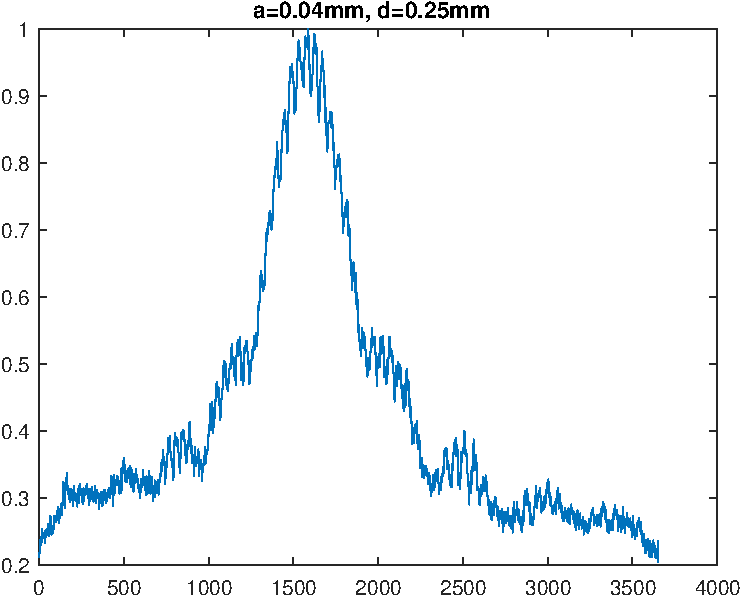
\includegraphics[width=1\linewidth,height=9cm]{04_y_25.pdf}\label{fig:A3}}
		\hfill
		\subfloat[Patrón de irradiancia teórico]{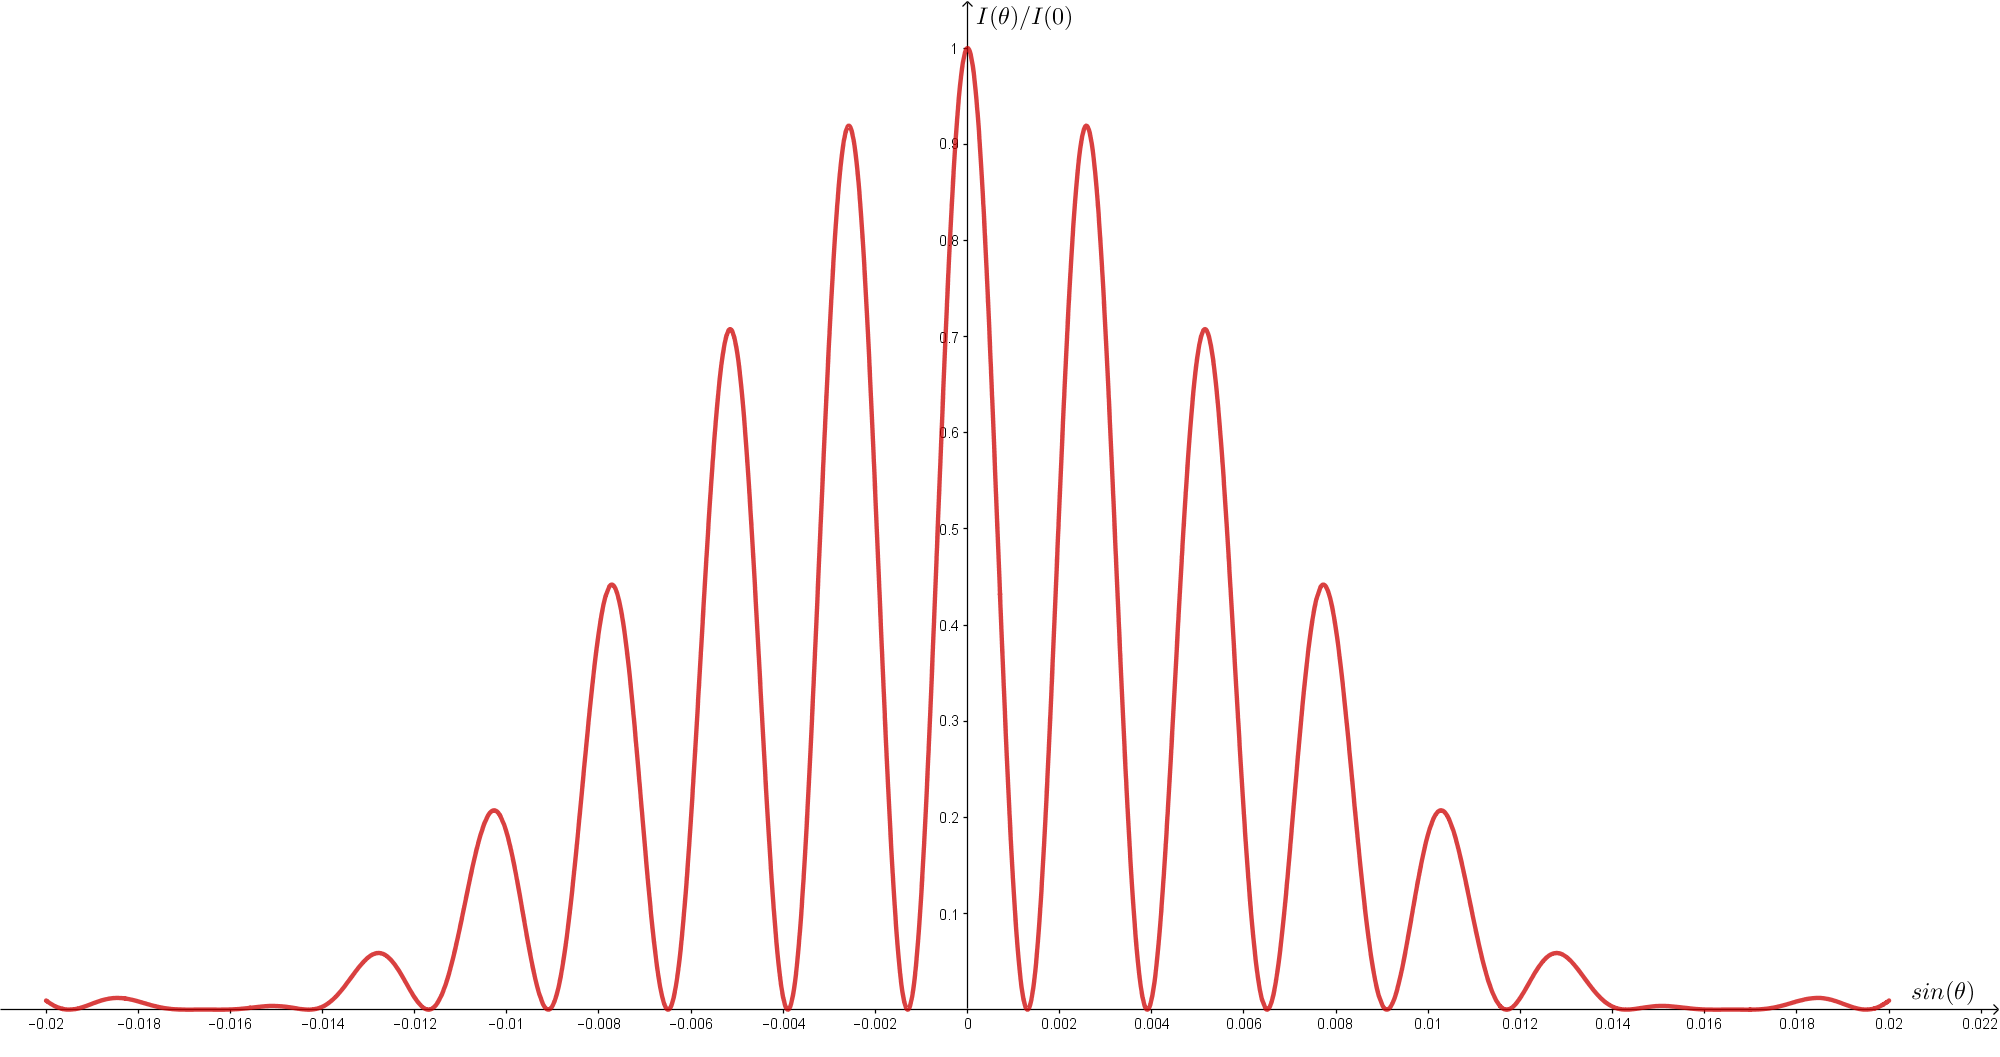
\includegraphics[width=1\linewidth,height=9cm]{Irradiancia 1.png}\label{fig:A2}}
		\hfill
		\caption{Patrones de irradiancia para la rendija indicada}
		\label{fig:P1}
	\end{figure}

	\begin{figure}[htbp!]
		\centering
		\subfloat[Foto de la rendija]{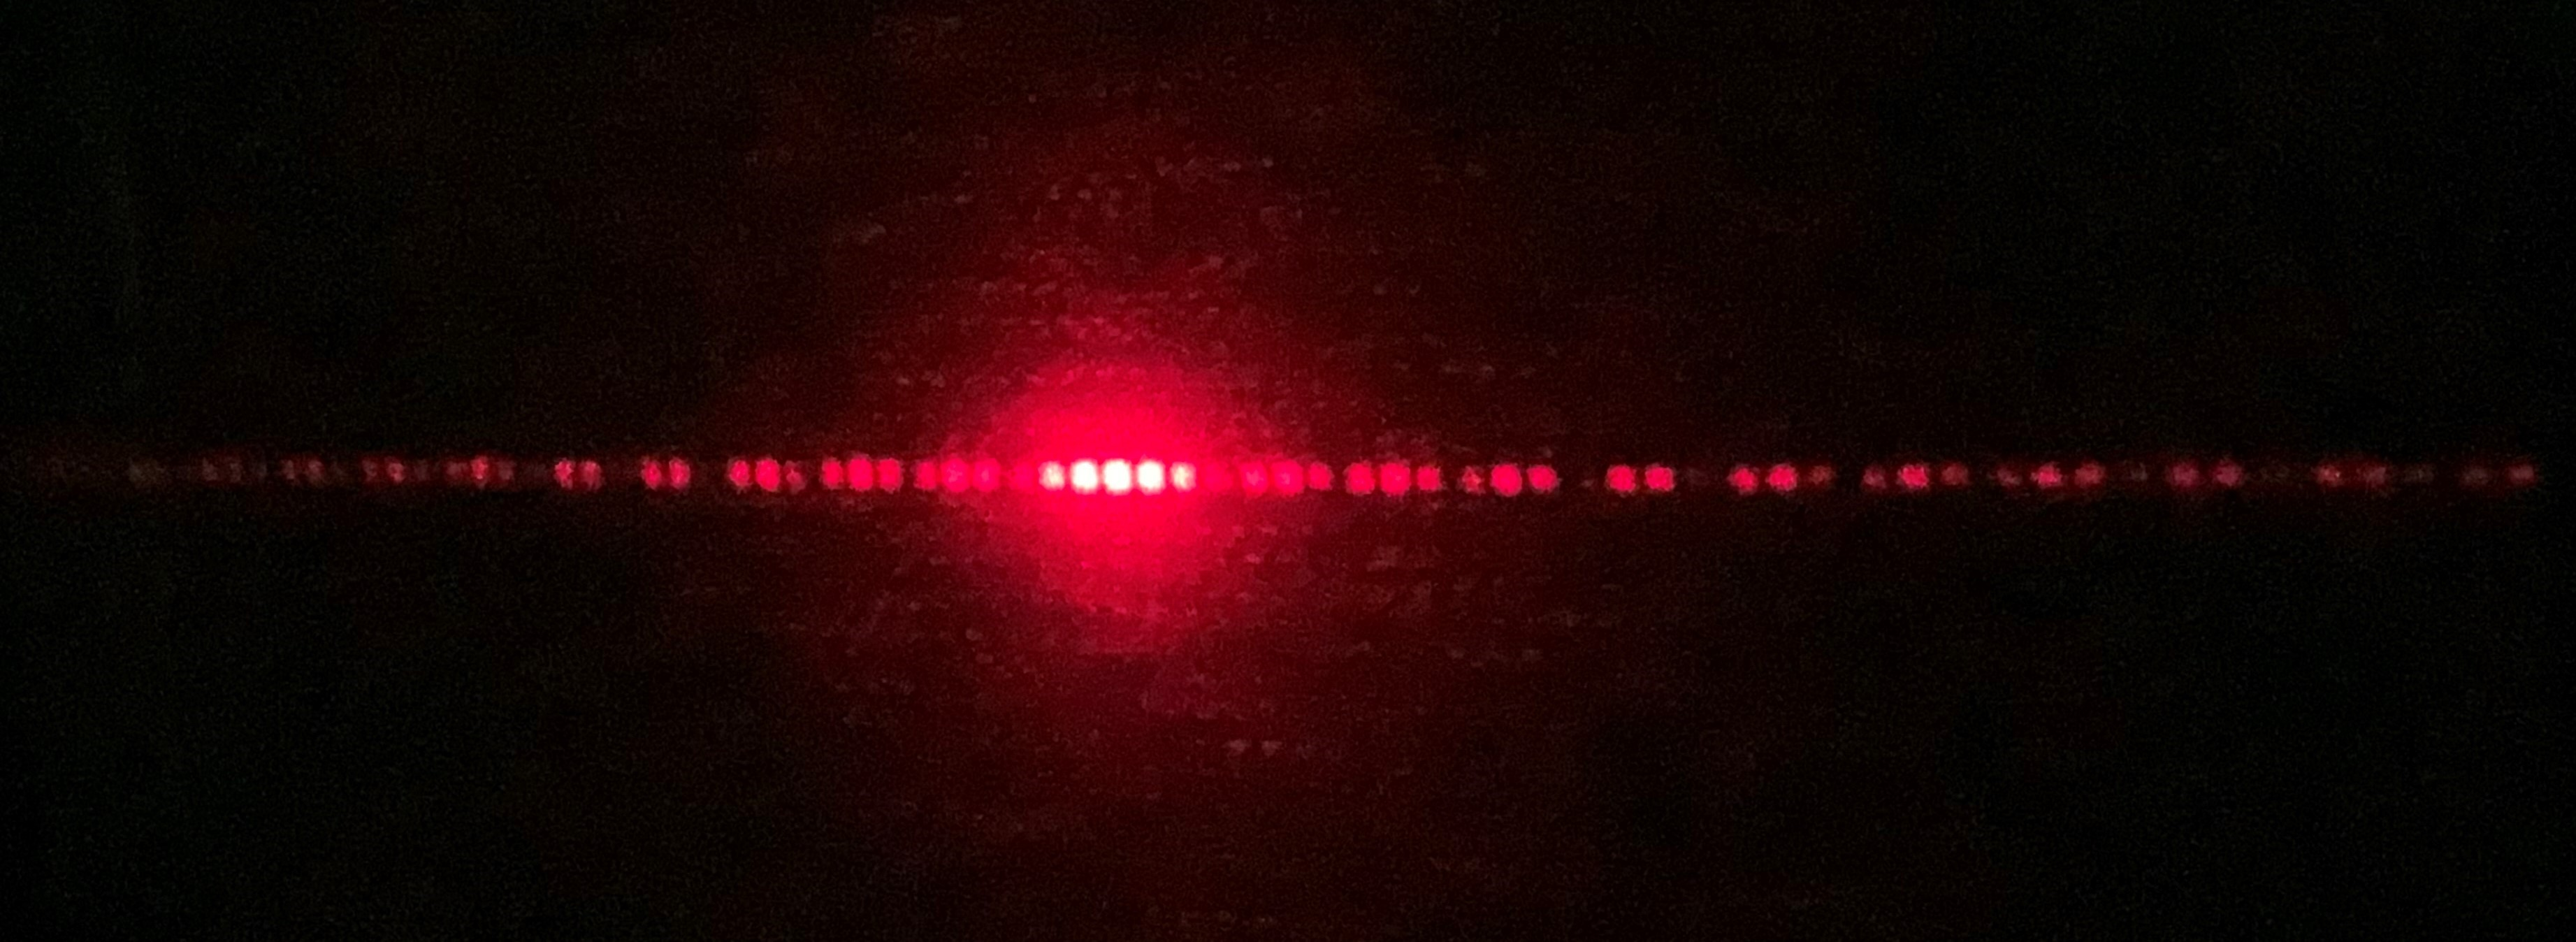
\includegraphics[width=1\textwidth, height=4cm]{08_y_25.jpg}\label{fig:A4}}
		\hfill
		\subfloat[Patrón de irradiancia experimental]{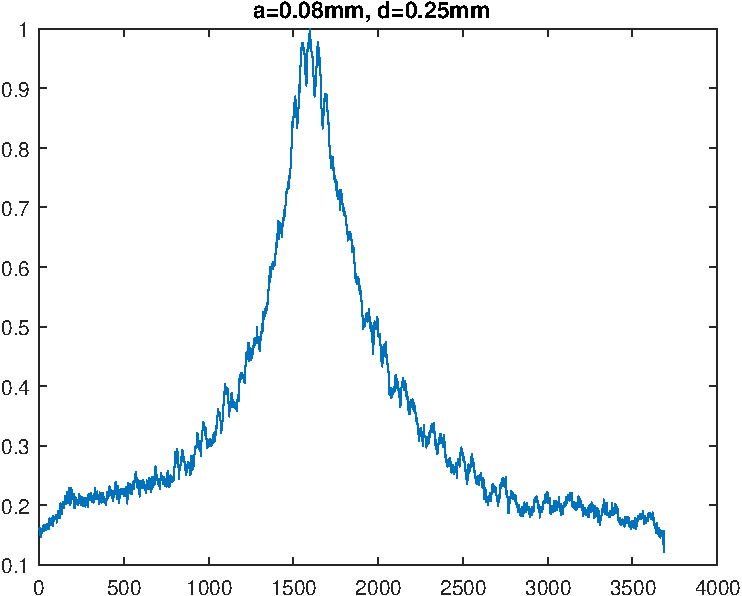
\includegraphics[width=1\linewidth,height=8.5cm]{08_y_25.pdf}\label{fig:A5}}
		\hfill
		\subfloat[Patrón de irradiancia teórico]{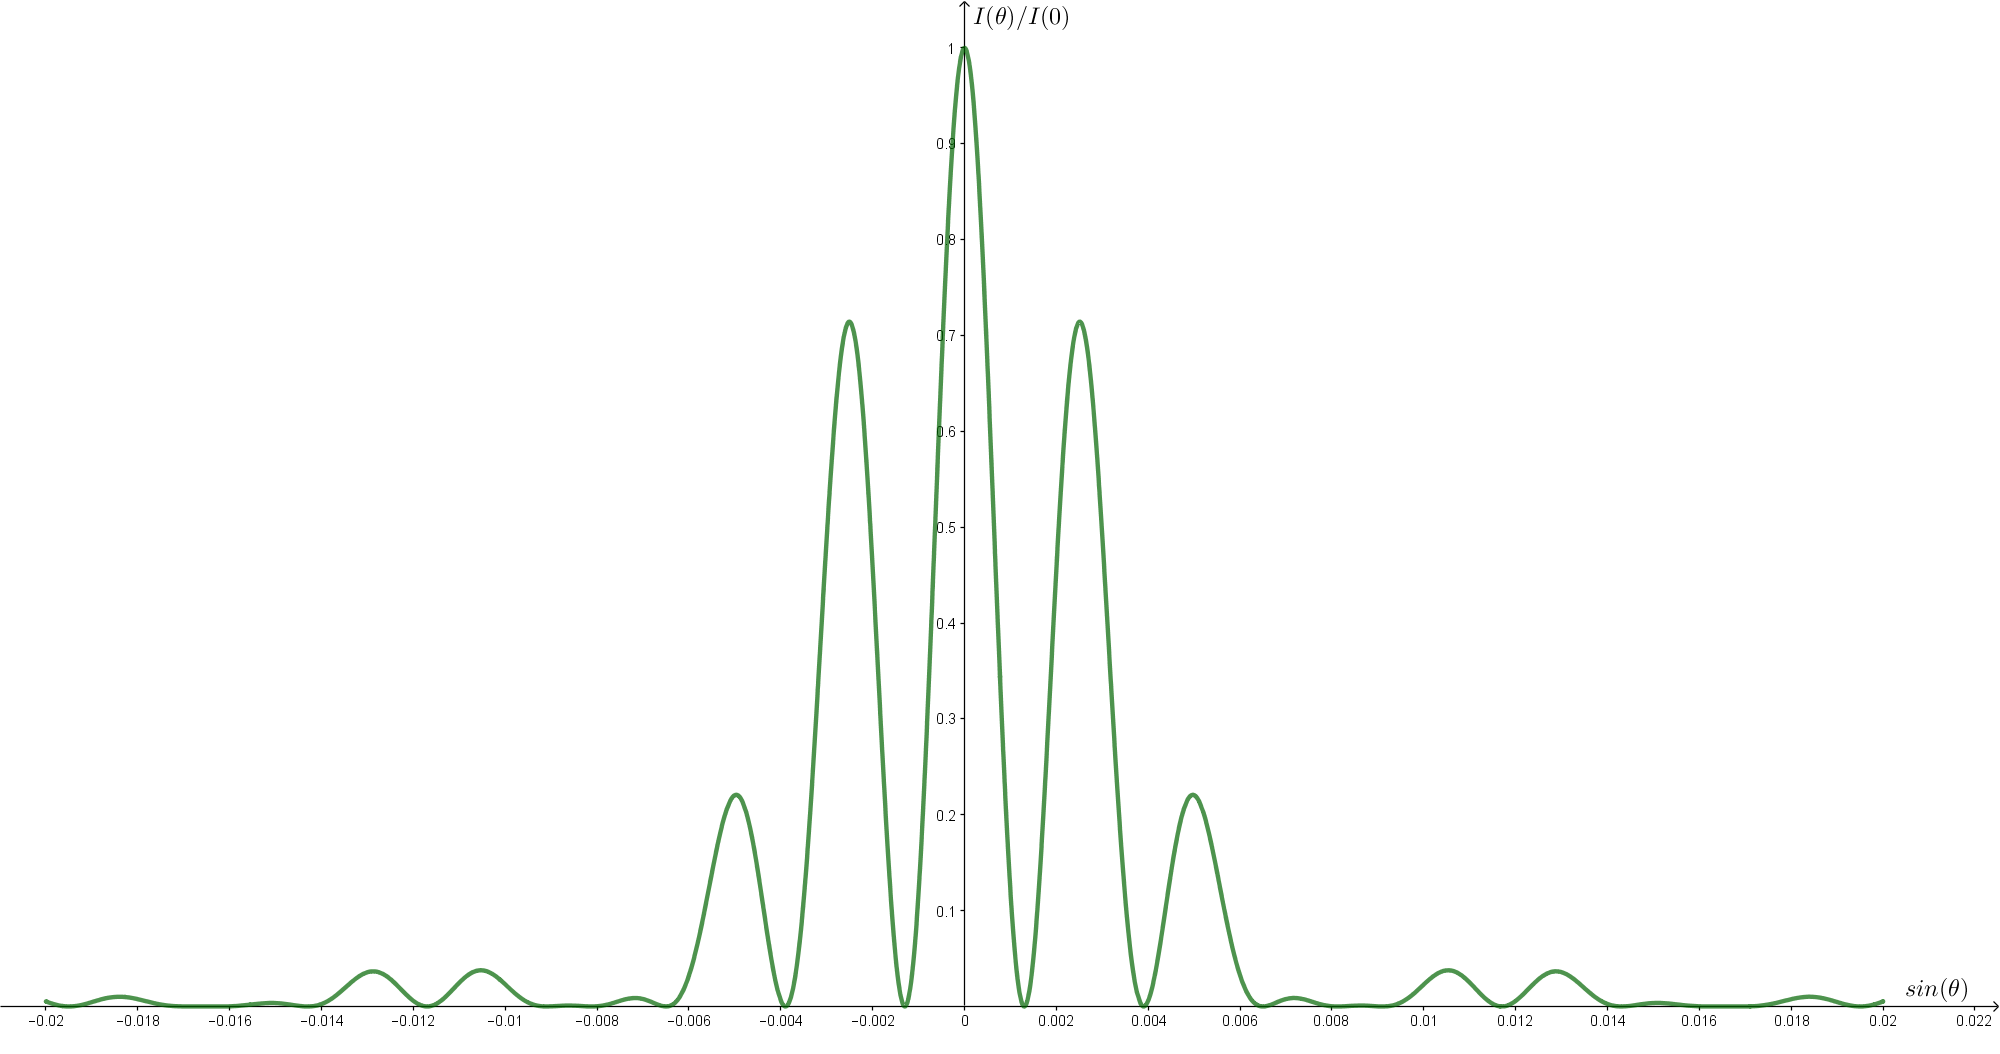
\includegraphics[width=1\linewidth,height=9cm]{Irradiancia 2.png}\label{fig:A6}}
		\hfill
		\caption{Patrones de irradiancia para la rendija indicada}
		\label{fig:P2}
	\end{figure}

	\begin{figure}[htbp!]
		\centering
		\subfloat[Foto de la rendija]{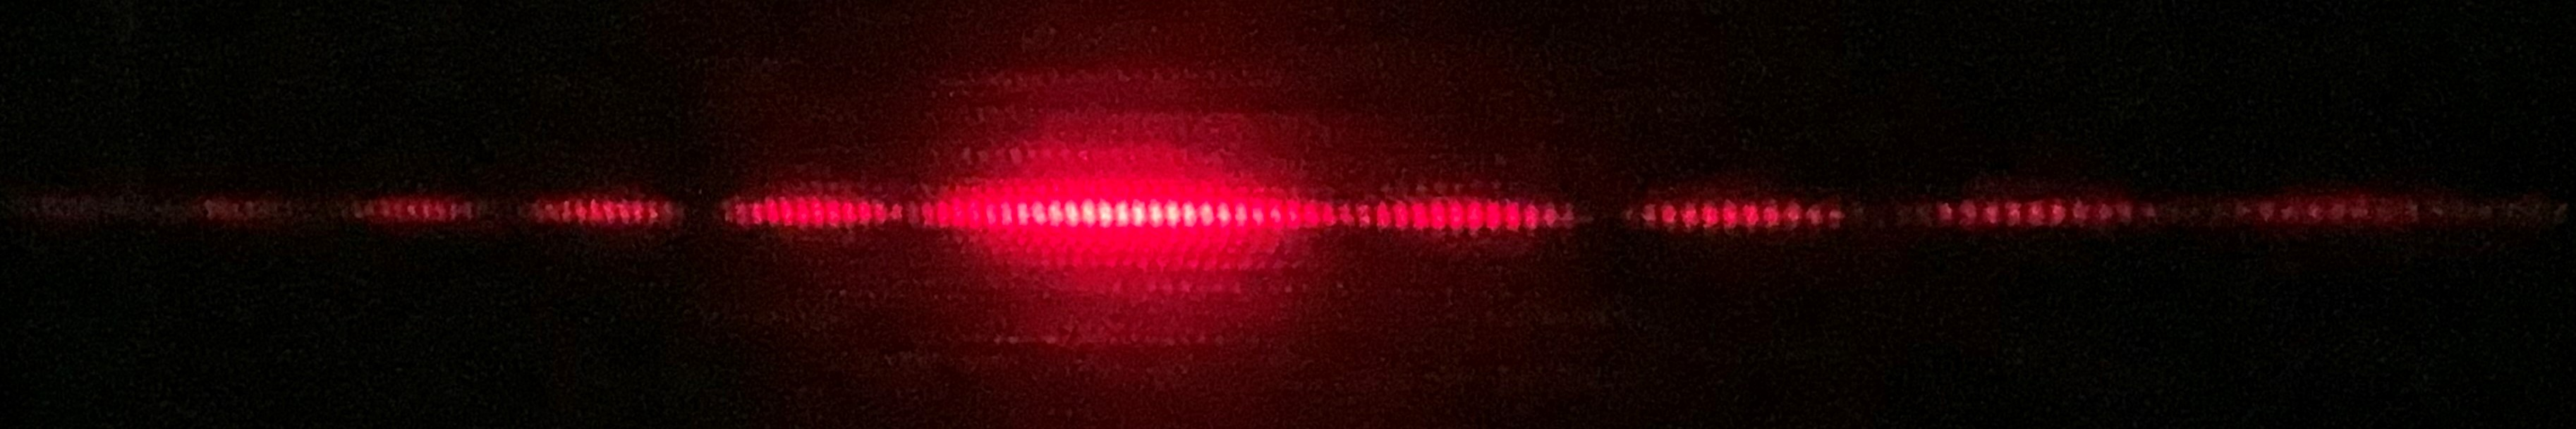
\includegraphics[width=1\textwidth]{04_y_5.jpg}\label{fig:A7}}
		\hfill
		\subfloat[Patrón de irradiancia experimental]{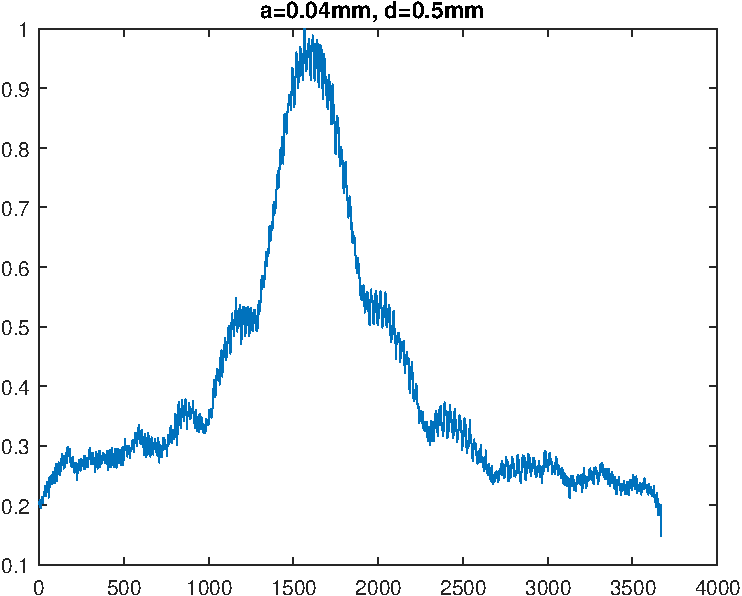
\includegraphics[width=1\linewidth,height=9cm]{04_y_5.pdf}\label{fig:A8}}
		\hfill
		\subfloat[Patrón de irradiancia teórico]{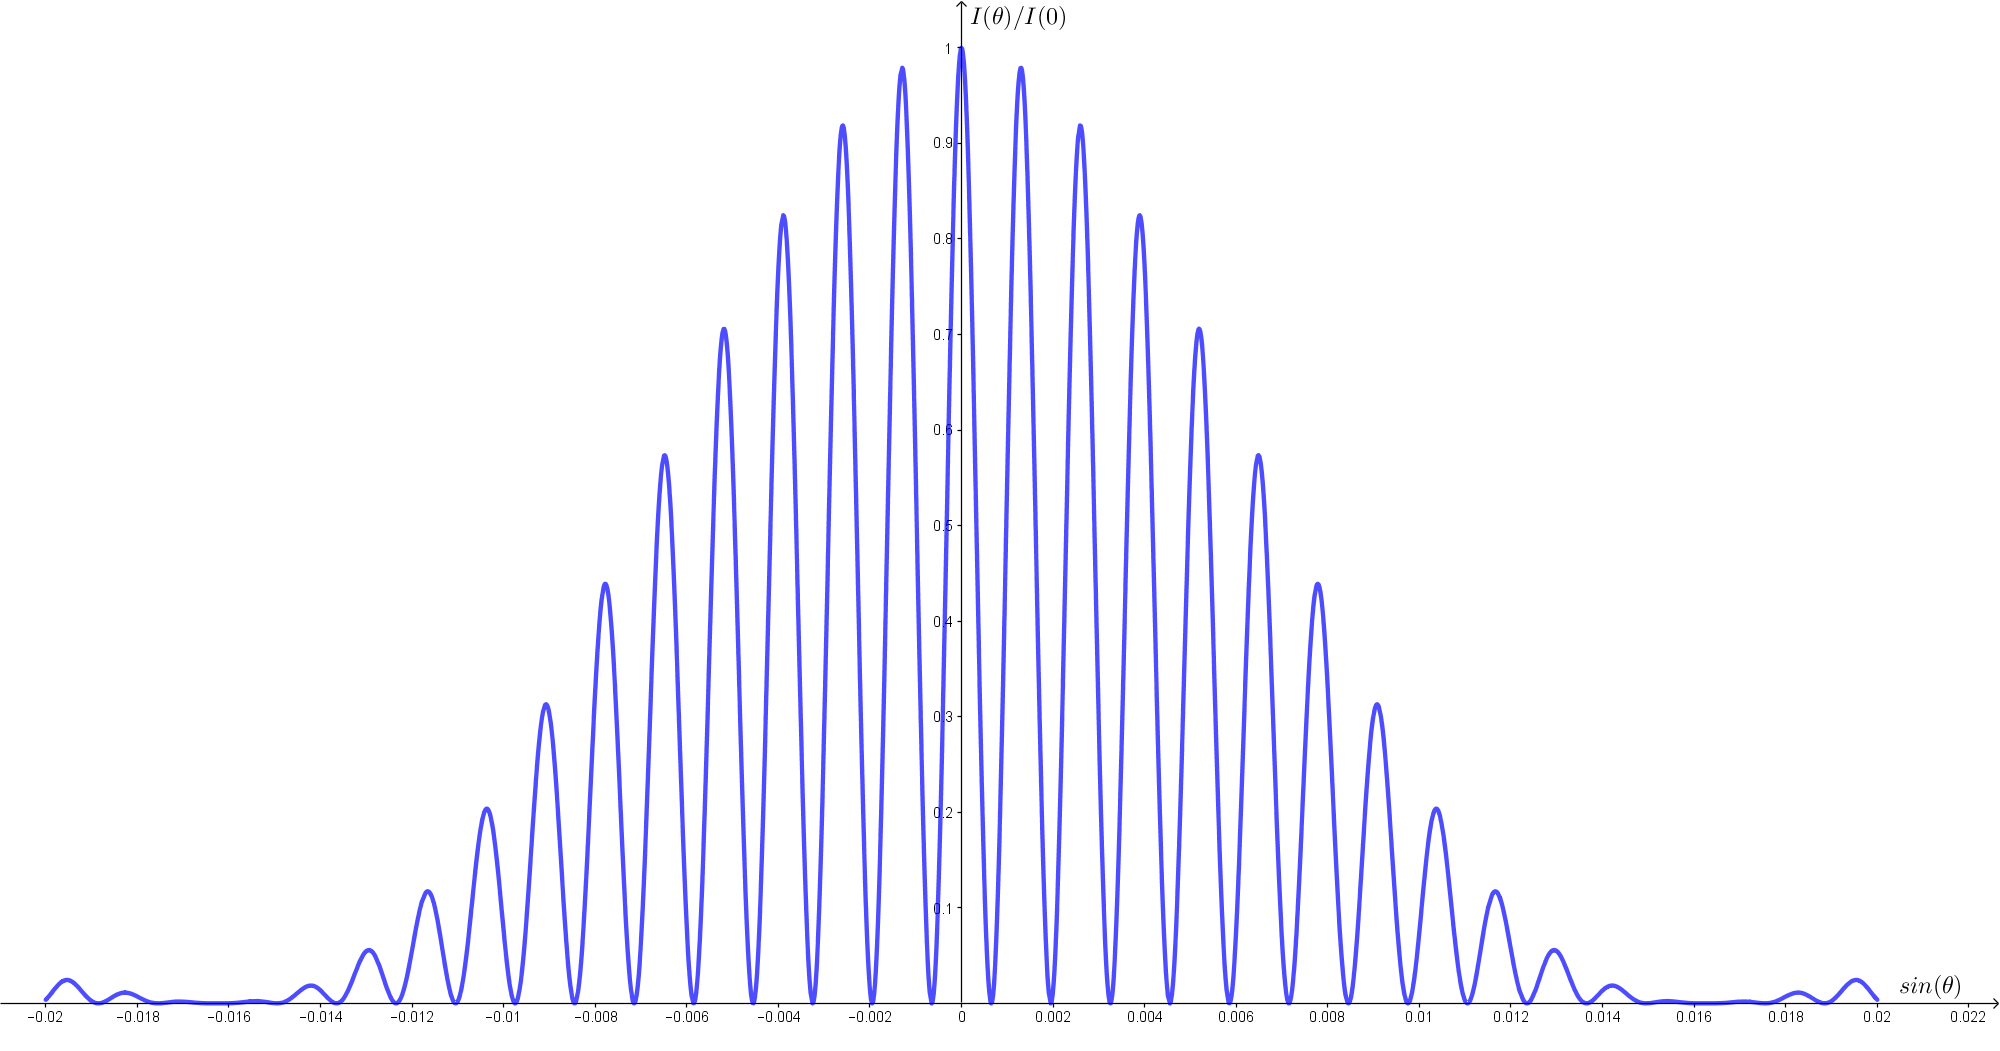
\includegraphics[width=1\linewidth,height=9cm]{Irradiancia 3.png}\label{fig:A9}}
		\hfill
		\caption{Patrones de irradiancia para la rendija indicada}
		\label{fig:P3}
	\end{figure}
	
	\begin{figure}[htbp!]
		\centering
		\subfloat[Foto de la rendija]{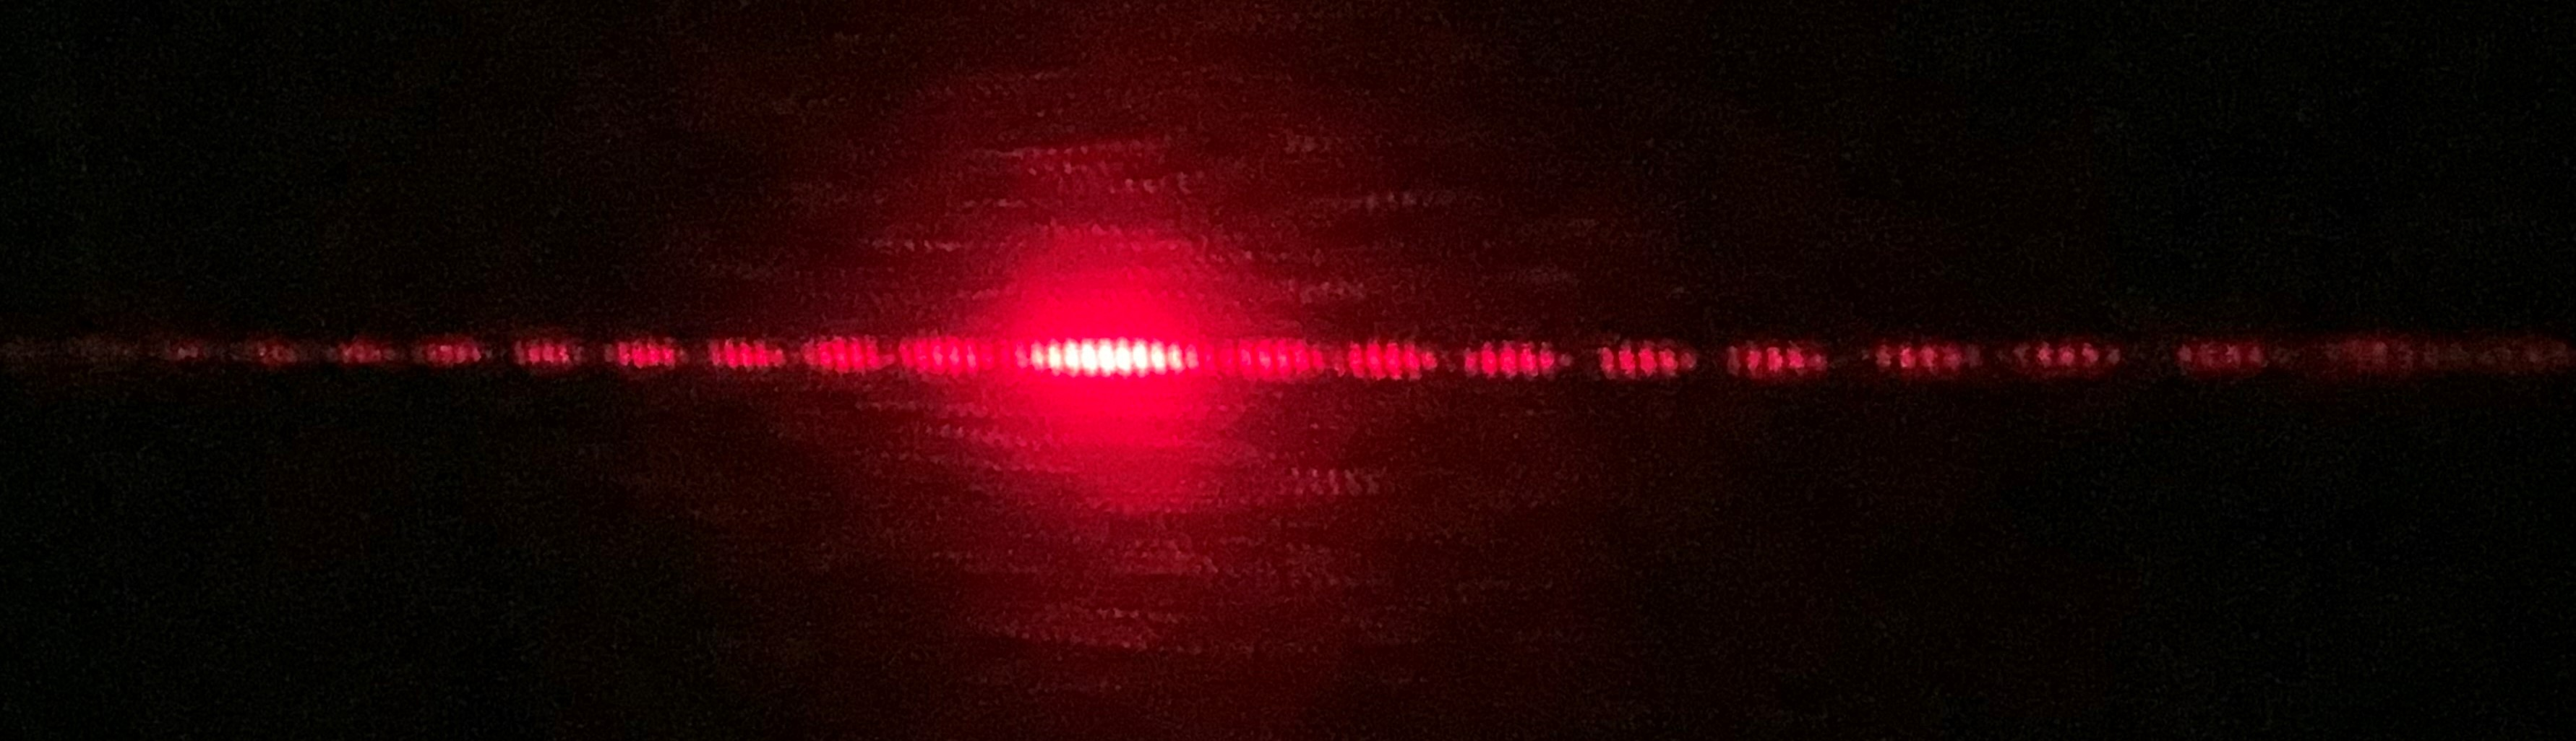
\includegraphics[width=1\textwidth, height=4cm]{08_y_5.jpg}\label{fig:A10}}
		\hfill
		\subfloat[Patrón de irradiancia experimental]{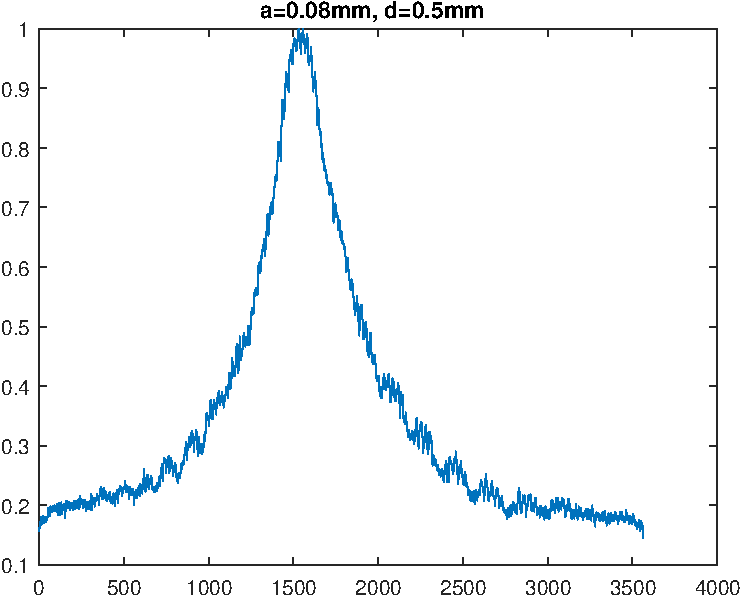
\includegraphics[width=1\linewidth,height=8.5cm]{08_y_5.pdf}\label{fig:A11}}
		\hfill
		\subfloat[Patrón de irradiancia teórico]{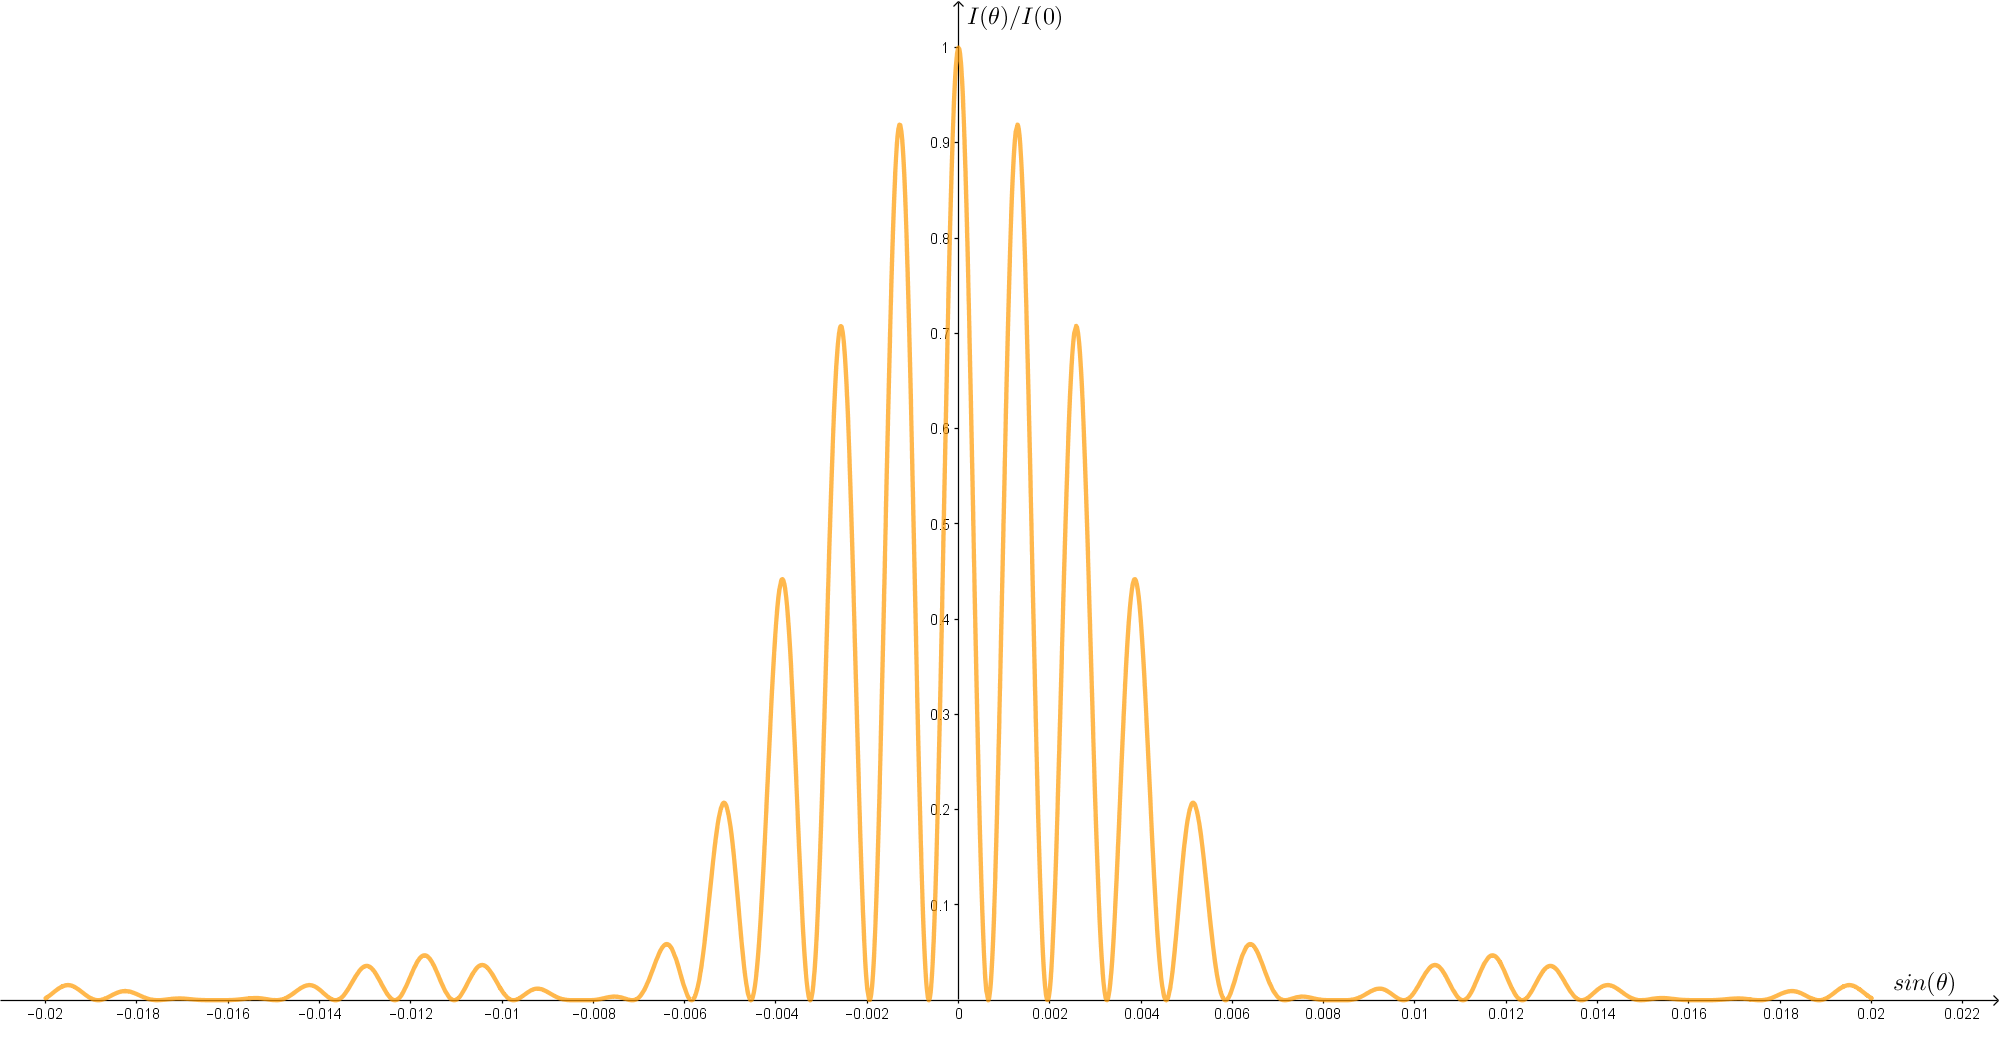
\includegraphics[width=1\linewidth,height=9cm]{Irradiancia 4.png}\label{fig:A12}}
		\hfill
		\caption{Patrones de irradiancia para la rendija indicada}
		\label{fig:P4}
	\end{figure}
		
	
\section{DISCUSIÓN DE RESULTADOS Y CONCLUSIONES.} % (((
% )))

% === REFERENCIAS === (((
% \bibliography{Referencias}
% \bibliographystyle{unsrt}
% )))

\section{APÉNDICE.} % (((
% )))

\subsection{--- Propagación de la Incertidumbre ---}
	
	La propagación de la incertidumbre para el producto y un cociente están dadas (respectivamente) por
	\begin{align*}
		(x\pm\delta x)(y\pm\delta y)&=x\cdot y\pm\left(|y|\delta x+|x|\delta y \right)\\\\
		\dfrac{x\pm\delta x}{y\pm\delta y}&=\dfrac{x}{y}\pm\left(\dfrac{\delta x}{|y|}+|x|\dfrac{\delta y}{|y|^2}\right)
	\end{align*}
	
	Para el caso particular en que $ y $ no posee incertidumbre, estas operaciones se simplifican a
	\begin{align*}
		(x\pm\delta x)(y)&=x\cdot y\pm|y|\delta x\\\\
		\dfrac{x\pm\delta x}{y}&=\dfrac{x}{y}\pm\dfrac{\delta x}{|y|}
	\end{align*} 

	\subsection{--- Cálculo teórico de las distancias entre máximos ---}	
	
	Haciendo uso de la fórmula \ref{} y los datos experimentales, se obtienen los siguientes cálculos
	\begin{itemize}
		\item Para $ d=0.25mm=0.025cm $

		\begin{align*}
			y_2&=\dfrac{2\cdot (6.5\times10^{-5}cm)\cdot[(90\pm 0.05) cm]}{0.025 cm}=
			\dfrac{(0.0117\pm 6.5\times 10^{-6}) cm^2}{0.025 cm}=
			(0.4680\pm 0.0002)cm\\\\
			y_4&=\dfrac{4\cdot (6.5\times10^{-5}cm)\cdot[(90\pm 0.05) cm]}{0.025 cm}=
			\dfrac{(0.0234\pm1.3\times 10^{-5})cm^2}{0.025 cm}=
			(0.9360\pm0.0005)cm\\
		\end{align*}
	
		\item Para $ d=0.5mm=0.05cm $
		
		\begin{align*}
			y_2&=\dfrac{2\cdot (6.5\times10^{-5}cm)\cdot[(90\pm 0.05) cm]}{0.025 cm}=
			\dfrac{(0.0117\pm 6.5\times 10^{-6}) cm^2}{0.05 cm}=
			(0.2340\pm 0.0001)cm\\\\
			y_4&=\dfrac{4\cdot (6.5\times10^{-5}cm)\cdot[(90\pm 0.05) cm]}{0.025 cm}=
			\dfrac{(0.0234\pm1.3\times 10^{-5})cm^2}{0.05 cm}=
			(0.4680\pm0.0002)cm\\
		\end{align*}	
		 
	\end{itemize}



\end{document}
